% \begin{figure}
%     \centering
%     \includegraphics[width=0.9\textwidth]{}
%     \caption{}
%     \label{fig:}
% \end{figure}

\chapter{Architectural Overview}
Figure \ref{fig:architectural_overview} shows a general architectural overview of the Demonstrator software.

\begin{figure}
    \centering
    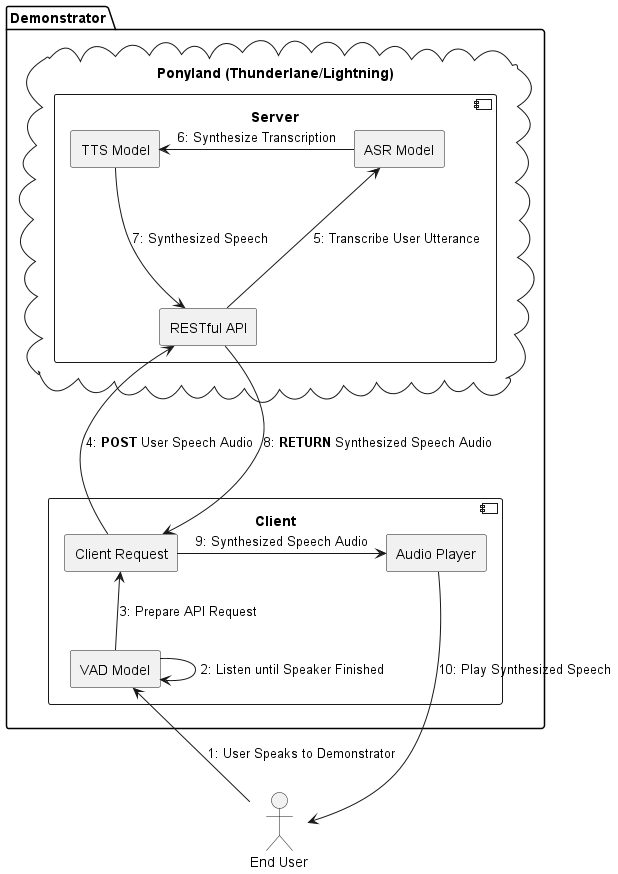
\includegraphics[width=0.9\textwidth]{../diagrams/deployment.png}
    \caption{Architectural overview of the Demonstrator}
    \label{fig:architectural_overview}
\end{figure}

The Demonstrator is a Python-based program and is primarily a cloud-based software that records records and process end user speech in order to communicate with the end user.
As such, the architecture of the default Demonstrator setup revolves and the usage of a client, a server, and the communications between the two.
The client's responsibility is to interact with the end user by detecting and recording their speech and by playing back speech of their own, and is designed to be a low-spec device that can communicate over the internet and has a microphone and speakers.
The server's responsibility is to perform the heavy work, such as running a set of neural networks to transcribe and synthesize speech, and to send the results of that work to the client.

The overview of figure \ref{fig:architectural_overview} also shows the general steps the Demonstrator takes during a full conversational turn.
They are as follows:
\begin{enumerate}
    \item An end user interacts with the Demonstrator client, which is running idle and waiting for any end user input.
    \item The VAD (Voice Activity Detection) model waits until it detects any end user speech. It opens an audio stream upon program start, but does not record or save this audio. When it detects that an end user has started speaking, it will start to record the speech until the end user has finished speaking, which is assumed to be after roughly 1,5 seconds of continuous silence.
    \item The client starts to prepare a POST request to the server's RESTful API.
    \item The client sends the POST request to the server, which includes the end user speech audio. The server then receives this audio, alongside any relevant additional information.
    \item The server runs the ASR (Automatic Speech Recognition) model on the end user speech audio to produce a transcription.
    \item The server runs the TTS (Text-to-Speech) model on the transcription to produce its own synthesized speech.
    \item The server starts to prepare a response for the client's request.
    \item The server sends the response, which includes the synthesized speech and some additional metadata about that speech. The client receives this information.
    \item The client plays back the synthesized audio using its audio player module.
    \item The end user hears the Demonstrator's speech.
\end{enumerate}

\chapter{Detailed Design Description}
This section of the SDD goes through the Demonstrator software in more detail.
The structure of this section reflects the folder hierarchy of the Demonstrator codebase in its current form, with the aim of making traversal of this document more straightforward.
This document will not contain all of the Demonstrator's code and their latest inline documentation, so for the full and up-to-date code and inline docs it is advised to look at the code itself.

\section{\texttt{configs}}
This folder contains files that should be used for configuring the Demonstrator.
These configurations should be relatively easy to read and alter, as they are meant to be used and read by developers and those wanting to use the Demonstrator.
For this reason, the human-readable YAML format is currently used for these configurations.

\subsection{\texttt{demonstrator\_configs.yaml}}
The \texttt{demonstrator\_configs.yaml} file contains the configuration for the Demonstrator setup.
These configurations hold true for all Demonstrator instances, so they are tracked in Git.
The file opens with some configuration variables that are independent of any type of Demonstrator.
Variables that are relevant to only clients, servers, and/or apps, are listed further below in their respective category.

The configuration variables that are relevant across Demonstrator types are:
\begin{itemize}
    \item seed: an integer used as the seed for functions that have an element of randomness. By using a set seed for these functions, the Demonstrator's outputs become more predictable. Used across libraries, including the random built-in, PyTorch, and HuggingFace.
    \item threads: the number of GPU threads the Demonstrator is allowed to use at the same time. Integer.
    \item host\_ip: the IP address of the server's RESTful API. Clients connect to this IP address on the port number provided in the host\_port variable.
    \item host\_port: the port number clients connect to. Appended onto the IP address of the host\_ip variable.
\end{itemize}

Afterwards, configuration for the Demonstrator types app, server, and client are defined.
These are defined in what are called \textbf{\textit{profiles}}.
A profile contains all the configuration variables needed to make an app, server, or client work.
A Demonstrator type can have multiple profiles, making switching between configuration setups easy and flexible.
However, \textbf{every Demonstrator type should at least have one profile named "default".}
These profiles are defined across all Demonstrator instances
The \texttt{/.env} file contains the specific profile used by an individual Demonstrator instance.

An example of defining profiles for a Demonstrator app looks like so:
\begin{lstlisting}
app:
    default:
        language: nl
        asr:
            name: whisper
            model_size: medium
        tts:
            name: mms
        vad:
            name: silero
    whisper_large_english:
        language: en
        asr:
            name: whisper
            model_size: large-v2
        tts:
            name: piper
        vad:
            name: silero
\end{lstlisting}

Lines with zero indentation define the Demonstrator type (app, server, client).

The first level of indentation defines a profile.
In this case, there are two profiles: "default" and a profile called "whisper\_large\_english".
These are the potential values that can be used in the \texttt{/.env} file's DEMONSTRATOR\_PROFILE variable.

At the second level of indentation, the things that should be configured are defined.
With the current support, these are, per Demonstrator type:
\begin{itemize}
    \item app: language, asr, tts, vad
    \item server: language, asr, tts
    \item client: vad
\end{itemize}
In this case, we define what ASR, TTS, and VAD models an app should use for this profile, alongside which language it should transcribe/synthesize in.
For the default profile, that is Dutch (nl), and for the "whisper\_large\_english" profile, it's English (en).

The third level of indentation are specific settings for the types of models that are used by that type of Demonstrator.
Currently, the following variables and values are supported:
\begin{itemize}
    \item asr: 
    \begin{itemize}
        \item name: currently in ["whisper",]. The ASR model that is used by the Demonstrator.
        \item model\_size: currently in ["tiny", "base", "small", "medium", "large-v2", "large-v3",], dependent on the model chosen in the \textit{name} variable. Defines the size of the ASR model.
    \end{itemize}
    \item tts:
    \begin{itemize}
        \item name: currently in ["mms", "piper",]. The TTS model that is used by the Demonstrator.
    \end{itemize}
    \item vad:
    \begin{itemize}
        \item name: currently in ["silero",]. The VAD model that is used by the Demonstrator.
    \end{itemize}
\end{itemize}
In the example, the default profile defines that we should use the FasterWhisper ASR model at size medium, the MMS-TTS model for TTS, and the SileroVAD model for VAD. The "whisper\_large\_english" instead defines a FasterWhisper ASR model at size large-v2, with the Piper TTS model for TTS, and the SileroVAD model for VAD.

The values assigned to the variables are read when running the Demonstrator.
This is done in the \texttt{/src/demonstrator.py} file by the DemonstratorFactory class.
Specifically, its parse\_model\_configs() method defines what variables are supported in a profile, what values they can hold, and how those values are translated into actual code.
\textbf{Should you want to change, add, or remove any of this functionality, this is where you can do so.}

\subsection{\texttt{eval\_configs.yaml}}
The \texttt{eval\_configs.yaml} file contains the configuration for the evaluation setup.
Currently, the evaluation suite only evaluates the ASR model by measuring its Word Error Rate (WER) and Real-Time Factor (RTF).
This is reflected in the existing evaluation configuration support.

One can define multiple evaluation setups and alternate between them when running the code in the \texttt{/eval} folder.
An example of an evaluation configuration is as such:
\begin{lstlisting}
asr_eval_no_edge_cases:
    manifest: asr_eval.json
    model_sizes:
      - tiny
      - base
      - small
      - medium
      - large-v2
    exclude:
      type: edge_case
\end{lstlisting}
The non-indented line defines what the evaluation configuration is called.
In this case, that's "asr\_eval\_no\_edge\_cases".

The first level of indentation defines the variables that should have a value.
They are as such:
\begin{itemize}
    \item manifest: the manifest to use. A manifest is a JSON file that exists in the \texttt{/data/manifests/} folder. It defines the evaluation dataset. The value here should be the full name of one of the manifest files in this folder, \textbf{including the file extension}. In the example here, we use the evaluation manifest \texttt{/data/manifests/asr\_eval.json}.
    \item model\_sizes: a list of the model sizes that are tested. Currently, these are the model sizes for the FasterWhisper model. In this example, we test FasterWhisper models at sizes tiny, base, small, medium, and large-v2.
    \item exclude: optional. If included, defines what data should be excluded from the evaluation. In the example, we exclude data points that have the type "edge\_case". These are utterances that are intentionally meant to throw off an ASR model's usual performance, such as laughter and interjections.
\end{itemize}

\section{\texttt{data}}
This folder contains all data relevant to the Demonstrator.
Since none of the Demonstrator's models are actually trained or finetuned on data, this mostly concerns evaluation data, files that are stored temporarily, and files that are read by the Demonstrator during runtime so that they aren't included in the codebase itself.

\subsection{\texttt{audio}}
Contains all audio data relevant to the Demonstrator.

\subsubsection{\texttt{eval}}
Contains the audio files used for the evaluation of the ASR model (in the \texttt{/eval/} folder).
These files are not tracked by Git, so they are not downloaded automatically on any new client installs.
However, they have been placed on the current Ponyland server install and can be accessed there.
The audio recordings are in .wav format and concern recordings made by the author of this document (me).
The files are named "\{semantic\_group\}\_\{number\}\_\{language\_code\}.wav", where "semantic\_group" is currently either "story", "emotion", or "edge\_case".
These audio files are part of the dataset defined in \texttt{/data/manifests/asr\_.json}, where every audio file's transcription can also be found.
Since this concerns personal data, \textit{please do not spread these audio's around for other purposes without my permission}.
Understandably, this may be an issue, and I would recommend replacing these recordings in their entirety in favor of more robust evaluation data that is publicly available.

\subsection{\texttt{manifests}}
Contains manifest files for the Demonstrator.
In this context, a manifest is a file that ties together various other files to create a coherent unit, often for defining datasets.
For example, there currently exists only one manifest in this repository called \texttt{/data/manifests/asr\_eval.json}, which defines the dataset used to evaluate the ASR model.
This manifest is a JSON file where every entry is one data record.
Every data record contains the relevant features and all data records together form a dataset.
This makes the manifest the definition of a dataset.
The main advantages of using manifests this way are that we can flexibly alter the contents and scope of the audio dataset and the audio data itself can be stored on disk as actual audio files instead of a different format, such as an array stored in a CSV file or binary data stored in a parquet file.

A data record of the \texttt{/data/manifests/asr\_eval.json} file looks like such;
\begin{lstlisting}
[
    {
        "filename": "edge_case_1_nl.wav",
        "transcription": "Hmm, eh, tja.",
        "type": "edge_case",
        "notes": "Filled pauses"
    },
]
\end{lstlisting}
and contains the following fields;
\begin{itemize}
    \item filename: the name of the audio file that should be included in the dataset. Must be a file that exists in \texttt{/data/audio/eval/}. Name must include the file extension.
    \item transcription: the transcription of the utterance heard in the audio. Used as the ground truth during evaluation.
    \item type: the category the utterance semantically belongs to. "story" means that the utterance tells (part of) a story, "emotion" means that the utterance is about someone guessing what emotion they just heard, and "edge\_case" are utterances meant to throw the ASR model off-guard.
    \item notes: optional. Any notes about the audio, such as why an utterance is labeled as an edge case. In the above example, the note says the utterance is an edge case since it contains only filled pauses.
\end{itemize}

\subsection{\texttt{tts\_messages}}
Contains JSON files that contain text used by the Demonstrator during inference.
Every file is named after one of the Demonstrator's supported languages, such as \texttt{data/tts\_messages/nl.json}, and contains the same set of messages translated into different languages.
Upon startup, the Demonstrator will refer to the file whose language matches the language used by the Demonstrator during that run, and uses that file's texts when pronouncing TTS messages.
This way, it is ensured that a Demonstrator will fully speak in the language specified.

These texts were originally included in the Demonstrator's codebase, but when expanding the Demonstrator's functionality to be multilingual, altering and expanding the TTS message texts for every supported language became cumbersome in the codebase itself.
That is why there now exists a specific place where these texts are stored.
Now, adding TTS support for a new language has become easier, and it is easier to alter any existing TTS messaging.

\section{\texttt{docs}}
Contains all documentation relevant to the demonstrator, including various documents, but also images and audio.

\subsection{\texttt{diagrams}}
Contains a collection of diagrams that explain the Demonstrator's functionality.
Currently, there is 1 diagram of the Demonstrator's general architecture, which is shown in figure \ref{fig:architectural_overview}, and 3 diagrams showing the program flow of a Demonstrator client, server, and app, as state machines.
These diagrams were made using PlantUML and both the PlantUML source code and the rendered image are included.

\subsection{\texttt{notes}}
Contains a collection of MarkDown files that contain notes written during internship meetings.
Every file is named after a date in the YYYY-MM-DD format, which reflects the date the meeting took place.

\subsection{\texttt{sdd}}
Contains this document.

\subsection{\texttt{installation\_client.md}}
The instructions for installing a Demonstrator client to a new PC.
These instructions should enable any end user to install the Demonstrator software to their PC so that they can use the Demonstrator either as a standalone app or as a client that connects with the Ponyland server.
This guide then assumes that the current installation on Ponyland is used as the server, but that is subject to change, given the current method of connecting to the server and where the installation is located.

\section{\texttt{env}}
Contains the Python environment for the Demonstrator.
It is not tracked using Git.
Although use of a local environment is recommended, it is not required.

\section{\texttt{eval}}
Contains files regarding the evaluation of the Demonstrator software.

\subsection{\texttt{results}}
Contains files with result data from an evaluation round.
Currently, there exist two files here: \texttt{asr\_eval.parquet} and \texttt{asr\_eval\_mean.parquet}.
\texttt{asr\_eval.parquet} contains the results from an evaluation round of the Demonstrator's ASR model for every data entry defined in the \texttt{/data/manifests/asr\_eval.json} manifest.
\texttt{asr\_eval\_mean.parquet} is the same, but contains the mean of every metric across all data entries.
Parquet files were chosen for storing results instead of CSV/TSV/JSON files due to their stability.
However, since they are stored as binary information, they cannot be opened to read their concents.
The results stored in these files can be easily viewed in the Jupyter notebook found in \texttt{/notebooks/evaluation\_results.ipynb}

\subsection{\texttt{eval.py}}
Contains the code for performing the evaluation of the Demonstrator.
Currently, there exists only evaluation for the ASR model by measuring performance using the Word Error Rate and Real-Time Factor, but any evaluations added in the future should be implemented here.
The current ASR evaluation function uses the manifest found in \texttt{/data/manifests/asr\_eval.json} to obtain an evaluation set and the configuration file in \texttt{/configs/eval\_configs.yaml} to determine which models should be tested, at what sizes, and if edge case data should be included in the evaluation or not.
It returns dataframes containing the evaluation data, with one dataframe containing metrics per data entry, and one dataframe containing metrics across the whole dataset.
These datasets are then stored as parquet files in \texttt{/eval/results/asr\_eval.parquet} and \texttt{/eval/results/asr\_eval\_mean.parquet} respectively.

\section{\texttt{notebooks}}
Contains (Jupyter) notebooks related to the Demonstrator project.
Currently, there is only one notebook, \texttt{evaluation\_results.ipynb}.

\texttt{evaluation\_results.ipynb} is a relatively straightforward notebook that aims to visualize the results of the latest evaluation round of the Demonstrator.
The evaluation data is stored as parquet files in \texttt{/eval/results/}, and since they are parquet files, they cannot be opened like CSV/JSON files could.
For this reason, the \texttt{evaluation\_results.ipynb} notebook loads in these evaluation data and shows them in a tabular manner.

\section{\texttt{src}}
The \texttt{src} folder contains all the code that implements the Demonstrator software, alongside some additional resources that are only relevant within the context of the program runtime.
Although it is currently called "src", it would be more standard to name this "demonstrator" or a similar package name.
However, this would require some refactoring in the codebase, so do keep that in mind.

The implementation of the Demonstrator was done in Python, so all code files mentioned here are written in Python.
Furthermore, most code is written in an object-oriented style, which was done for varying reasons (separation of concerns, code encapsulation, ease of altering runtime configuration, etc.).
As a result, it is recommended that anyone planning on continuing the Demonstrator's development is familiar with an object-oriented writing style and the terms associated with it, such as (abstract) classes, objects, methods, inheritance, etc.
These terms are also used in this part of the documentation.

\subsection{\texttt{models}}
Contains code that implements the various models used by the Demonstrator.
Currently, these include the VAD, ASR, and TTS models, but could also include implementations for LLMs and emotion detection models in the future.

\subsubsection{\texttt{asr.py}}
Contains the implementation for any ASR model that the Demonstrator can use.

The base class for any ASR model is called "ASRModel".
This is an abstract class that inherits from the AbstractModel class from \texttt{/src/models/model.py}, and although it has methods, they are also abstract.
The ASRModel class is, then, not an actual implementation of any specific ASR model, but more so a framework into which all actual implementations should fit.
If all implementations of an ASR model can be expected to all achieve the same end goal in the same way, then it is easy to switch between them (polymorphism), and the rest of the program does not need to worry about any specifics of how a specific ASR model works or differs from the others (separation of concerns).

The ASRModel base class has two abstract methods: "transcribe" and "warmup".
The transcribe method transcribes the audio passed to it in the language chosen in the configuration.
The warmup method is used once at program startup: it loads the ASR model into memory and lets it transcribe a brief utterance before an end user can interact with it.
This is done because the first transcription upon startup takes longer than subsequent transcriptions.
By transcribing a brief utterance before any end user input is processed, that extra loading time does not affect the end user.

There is currently one implementation of the ASRModel class, the "FasterWhisper" class, which implements the use of the faster-whisper model into the Demonstrator.
It is a multilingual neural model that automatically transcribes to the target language specified in the configuration found in the \texttt{/configs/demonstrator\_configs.yaml} file.
It also accepts speech input in a different language, but will then translate it internally and produce a translated transcription in the target language.
For example, English speech will be transcribed in Dutch if Dutch is the selected target language.

\subsubsection{\texttt{model.py}}
Contains the definition of the "AbstractModel" class, which is the parent class to all abstract classes of the types of models used by the Demonstrator (ASRModel, TTSModel, VADModel, etc.), and, by extension, all implementations of models.
This class exists so that it can be given properties that are useful for all types of models, which are then inherited by all model implementations.
For example, the AbstractModel has an instance of the MetricTracker class from \texttt{/src/metrics.py}, which tracks metrics of a model during inference, such as the Real-Time Factor.
By assigning a MetricTracker instance to the AbstractModel class, all ASR, TTS, and VAD models will automatically track relevant metrics during runtime.

\subsubsection{\texttt{tts.py}}
Contains the implementation for any TTS model that the Demonstrator can use.

The base class for any TTS model is called "TTSModel".
This is an abstract class that inherits from the AbstractModel class from \texttt{/src/models/model.py}, and although it has methods, they are mostly abstract.
The TTSModel class is, then, not an actual implementation of any specific TTS model, but more so a framework into which all actual implementations should fit.
If all implementations of a TTS model can be expected to all achieve the same end goal in the same way, then it is easy to switch between them (polymorphism), and the rest of the program does not need to worry about any specifics of how a specific TTS model works or differs from the others (separation of concerns).

The TTSModel base class has two methods: the abstract "synthesize" method and the implemented method "say\_goodbye".
The synthesize method accepts a piece of text and returns a synthesized speech of the text using the TTS model.
The say\_goodbye method is called when shutting down the program through the speech interface.
When shutting down this way, the Demonstrator will say one of a variety of goodbye messages to the end user before shutting down, which it does by calling this method.

There are currently two implementations of the TTSModel class: the "MMS" class and the "Piper" class, which respectively use the MMS-TTS and Piper TTS models for synthesizing speech.
The MMS class uses an end-to-end neural model to synthesize speech and supports many languages.
Because it is end-to-end, its vocal characteristics cannot be selected in advance, and may even fluctuate during inference, such as the sex perceived in the voice.
The Piper class uses a smaller neural model alongside a file that must be loaded from disk manually, which is stored in \texttt{/src/resources/models/}.
The Piper TTS can use different voices for the same language, so the perceived speaker sex and cadence are customizable.

\subsubsection{\texttt{vad.py}}
Contains the implementation for any VAD model that the Demonstrator can use.

The base class for any VAD model is called "VADModel".
This is an abstract class that inherits from the AbstractModel class from \texttt{/src/models/model.py}, and although it has methods, they are abstract.
The VADModel class is, then, not an actual implementation of any specific VAD model, but more so a framework into which all actual implementations should fit.
If all implementations of a VAD model can be expected to all achieve the same end goal in the same way, then it is easy to switch between them (polymorphism), and the rest of the program does not need to worry about any specifics of how a specific VAD model works or differs from the others (separation of concerns).

The VADModel base class has one abstract method called "listen".
An implementation of the listen function should open up a stream of audio input and continuously detect any end user speech.
If such speech is detected, it should start recording that speech until the end user has finished speaking.
This speech is then passed to the ASR model for transcription.

There is currently one implementation of the VADModel, which is called "SileroVAD", and uses the Silero VAD model for detecting speech.
This model processes the audio input in small chunks and estimates for every chunk a likelihood of speech being present in that chunk.
If its estimated likelihood exceeds a certain threshold, it is assumed that an end user has started speaking, and the audio is recorded.
Recording ceases when the estimated likelihoods are blow the threshold for a set amount of subsequent chunks.

\subsection{\texttt{resources}}
Contains various files that are relevant to the Demonstrator during runtime.
Currently, there are two subfolders that contain these files.

The first subfolder, \texttt{src/resources/audio}, contains audio files that are only relevant within the context of inference.
Examples of this are the audio file that is transcribed during warmup of the ASR model (see \texttt{src/models/asr.py}) and the temporarily stored files containing the latest end user utterance and latest TTS synthesized utterance.

The second subfolder, \texttt{src/resources/models}, contains model files that are loaded in from disk.
Currently, that only includes files related to the Piper TTS system.
This also means that this is the place where one can add new Piper TTS models.
\textbf{This subfolder isn't tracked by Git, so be aware of that for fresh installs!}

\subsection{\texttt{demonstrator.py}}
Contains the implementations for the different types of Demonstrators: clients, servers, and apps.
In total, there are currently 5 classes that occupy this file, which are as follows:
\begin{itemize}
    \item "Demonstrator": the base class for all types of Demonstrators.
    This is an abstract class that is implemented by any type of Demonstrator.
    Having this base class ensures that all Demonstrator types have some features that are relevant regardless of the Demonstrator type.
    These are things such as having a state, storing the latest end user utterance, and the "run" method.
    The run method works identically across Demonstrator types: in an indefinite loop, it simply calls a state object assigned as a class field and tells it to "handle" the current logic.
    This means that, at any moment, the logic of a Demonstrator is defined in the state that it's in.
    This makes the Demonstrator work like a state machine, which has many advantages: it is clear what every state does and what states the Demonstrator can advance to next, and it is easy to integrate new features into the Demonstrator by assigning them to a new state and connecting that state to an existing state.
    This improves predictability, maintainability, and extendability of the software.
    What states there are and what they do is discussed in the \texttt{/src/state.py} section, alongside the respective state machines of the Demonstrator types.
    \item "DemonstratorClient": an implementation of the Demonstrator that serves as the client in the client-server setup.
    \item "DemonstratorServer": an implementation of the Demonstrator that serves as the server in the client-server setup.
    \item "DemonstratorApp": an implementation of the Demonstrator that serves as a standalone application.
    \item "DemonstratorFactory": a class that creates Demonstrator instances based on the configurations in the \texttt{/configs/demonstrator\_configs.yaml} and \texttt{.env} files.
    On program startup, a DemonstratorFactory creates a Demonstrator instance based on the mode specified in \texttt{.env}.
    The models used by the instance are defined in the YAML configs as a profile, with the selected profile being read from \texttt{.env}.
    \textbf{Options for the configuration file are thus parsed here, and if one wants to add support for new configuration options, then this is where that support should be added. 
    Specifically, this is done in the "parse\_model\_configs" method.}
    The "create\_demonstrator" method then creates and returns the actual Demonstrator instances.
\end{itemize}

\subsection{\texttt{main.py}}
The entry point for the Demonstrator program.
It contains all code that happens when starting up the program.
Currently, that includes:
\begin{enumerate}
    \item Reading the values in the \texttt{.env} file to obtain the desired Demonstrator type and profile to use.
    \item Setting runtime conditions, such as the device on which to run models.
    \item Creating the DemonstratorFactory instance (see \texttt{/src/demonstrator.py}).
    \item If the instance it's running is a server, opening up an API endpoint \textit{on a separate thread}.
    \item Running the Demonstrator instance created by the DemonstratorFactory.
\end{enumerate}

\subsection{\texttt{metrics.py}}
Contains code related to the calculation and defining of metrics.
It contains the "MetricTracker" class, which is a class that is assigned to all models used by the Demonstrator to automatically track their metrics during inference.
Currently, it tracks the Real-Time Factor (RTF) for all models, and the Word Error Rate (WER) for ASR models during evaluation.
The Real-Time Factor is a measure of how time-efficient a model was in its calculation and expresses the speed at which a model can process an input of a certain size.
The Word Error Rate is a measure of accuracy for speech and describes how accurately the transcription provided by the ASR model matches with the actual transcription of t he utterance.
It thus has methods that called for calculating RTFs and WERs, alongside methods for calculating the mean of these metrics.

Aside from the MetricTracker, there are also separate functions that define how the WER and RTF are calculated.
These are explicitly not part of the MetricTracker class, so that they can be called without needing to instantiate a MetricTracker object first.
I would recommend this separation of concerns to any future developers: when adding new metrics, define the metrics themselves as separate functions that can be called wherever one needs to calculate it, and then give the MetricTracker class a method that uses that function to calculate the metric for the latest conversational round and store it.

\subsection{\texttt{playback.py}}
Contains code related to playing back audio to an end user.
The "PlaybackModule" class is an object owned by a Demonstrator client or app that can play back audio given to it using the speakers of the device it's running on, which it does by calling the "playback" method.

\subsection{\texttt{rest\_api.py}}
Contains the code that defines the RESTful API and its endpoints.
A Demonstrator server's API is implemented using the FastAPI library and currently has 2 endpoints.
These endpoints are defined as private functions at the bottom of this file and are called from \texttt{/src/main.py} when the Demonstrator starts to create the API.
This is not the standard approach offered by FastAPI, but it's done this way so that the endpoints can be implemented in a file separate from the file where they are called, which is the standard approach.
The standard setup would mean that all endpoints would have to be defined in the \texttt{/src/main.py}, while this approach separates concerns.
The endpoints are defined in the following functions:
\begin{enumerate}
    \item "\_API\_root": GET request to root ("/"). Home endpoint of the API, which returns a "Hello World!" message to the client if it successfully connected.
    \item "\_API\_user\_speech": POST request to "/user-speech". This endpoint receives audio files (files of type "audio/mpeg") containing the end user utterance, so that it can pass it to the ASR model for transcription.
    Once a POST request has been received, it will wait to give a response until the ASR models has finished transcribing and the TTS model has finished synthesizing.
    Only then will a response be sent containing the speech audio synthesized by the TTS model, with the HTTP code 201 CREATED signifying the successful synthesis of the utterance.
    This response will also contain metadata about the synthesized speech in the response headers, such as the audio length and its transcription.
\end{enumerate}

In addition to the endpoint functions, this file also contains a function called "send\_user\_speech\_request".
This function is called whenever a Demonstrator client instance wants to send an end user utterance to the server.
It sends a POST request to the endpoint defined in \_API\_user\_speech with the latest end user utterance audio attached and wait for a response.
This function is then also an example of how one can perform post requests to a FastAPI endpoint with a file attached.

\subsection{\texttt{runtime.py}}
Contains code that is used for controlling the runtime of the Demonstrator software.
This is a collection of mostly separate functions, but they all affect the runtime and are grouped under that moniker.
The file currently contains 4 functions:
\begin{itemize}
    \item "set\_universal\_seed": sets the same seed across multiple libraries that use randomness, such as the "random" built-in module, PyTorch, and HuggingFace.
    This is to improve reproducibility and predictability of the Demonstrator.
    The seed that is used can be found and altered to one's liking in the configuration file \texttt{/configs/demonstrator\_configs.yaml} under the "seed" variable.
    \item "set\_universal\_max\_threads": sets the maximal number of threads that a library can use concurrently.
    This is currently used to limit the number of threads a PyTorch model can take up concurrently.
    The number of threads allowed is set in the \texttt{/configs/demonstrator\_configs.yaml} configuration file under the variable "threads".
    \item "get\_cuda\_device": determines what device the Demonstrator's ASR and TTS models should run on.
    If no CUDA device is available, it returns "cpu" and the models are run on the CPU.
    If one CUDA device is available, it returns "cuda" and the models are run on the GPU.
    If more than one CUDA device is available, it calls the private function "\_get\_cuda\_device\_with\_most\_free\_memory", which looks through all available CUDA devices and selects the one with the most \textit{free} memory at that moment.
    The models are then run on this GPU.
    \item "\_get\_cuda\_device\_with\_most\_free\_memory": a private function that looks through all available CUDA devices and returns the one the larges amount of \textit{free} memory.
\end{itemize}

\subsection{\texttt{state.py}}
Contains code defining the various states a Demonstrator instance can be in.

The bulk of a Demonstrator instance's behavior is defined in the state that it's currently in.
This also means that, preferably, \textbf{new Demonstrator behavior should be implemented as a state.}
By using states as a way of defining the Demonstrator's behavior, the Demonstrator essentially becomes a state machine.
This has many advantages: it is clear what logic is performed and behavior is exhibited for every possible state a Demonstrator can be in,  what states the Demonstrator can advance to next, and it is easy to integrate new features into the Demonstrator by assigning them to a new state and placing that state into the existing state machine.
This improves predictability, maintainability, and extendability of the software.
The state machines for Demonstrator apps, clients, and servers can be found at the end of this section.

States are defined as classes.
To assign a state to a Demonstrator instance, an instance of that state class is created and assigned to the Demonstrator's "state" field (see \texttt{/src/demonstrator.py}).
The type of this field is "AbstractState".
The "AbstractState" is an abstract class and the parent class of all actual states.
The goals of the AbstractState is not to be instantiated and assigned to a Demonstrator, but to make sure that the every state class works in the same way.
This polymorphic design ensures that a Demonstrator instance never has to worry about what happens under the hood (separation of concerns) and can switch between all possible states without an issue, since they are all compatible due to a shared design and shared constraints (Liskov substitution principle).

The shared design in question is the use of the "handle" function.
The AbstractState has only one function called "handle", which "handles" the state logic.
This function is abstract for the AbstractState, and every actual state must implement it.
This implementation is then the behavior that the state should exhibit.
For example: a "Transcribe" state should implement the "handle" function to transcribe end user speech, and a "Synthesize" state should implement the "handle" function to synthesize audio using the TTS model.
Finally, all implementations of a state should end with assigning a new state to the Demonstrator (otherwise the state machine would run at a dead end).
The Demonstrator instance is passed as a parameter to the "handle" function and is called "context", since it is the context that these states run in.
This is a dependency injection approach and makes the Demonstrator instance loosely coupled from its states and their logic, which improves separation of concerns significantly.

The list of actual states a Demonstrator can be in, and thus all other classes that currently exist in this file, are as follows:
\begin{itemize}
    \item "Wakeup": the initial state all Demonstrator instances start in.
    The only logic it contains is assigning a different state to the Demonstrator instance, since not all Demonstrators want to exhibit the same behavior on startup: clients want to start listening to end user speech, while servers want to warm up their ASR models.
    \item "Warmup": prepares the ASR models of Demonstrator servers and apps by loading them into memory and making them transcribe a simple, prerecorded utterance.
    This is to ensure that the ASR model is ready to go once it receives an actual end user utterance.
    \item "Listen": makes the Demonstrator instance listen to input audio and record any utterances.
    The VAD model's Real-Time Factor is calculated here.
    \item "Transcribe": instructs the Demonstrator instance to transcribe a user utterance.
    The ASR model's Real-Time Factor is recorded here.
    A copy of the transcription is also preprocessed and compared to the string that activates the `SayGoodbye` state, and if they are the same, the program will move to that state.
    Otherwise, it will start to synthesize the transcription.
    \item "Synthesize": instructs the Demonstrator instance to synthesize the transcription provided to it.
    The TTS model's Real-Time Factor is also calculated here.
    \item "Speak": instructs the Demonstrator instance to play back the synthesized audio to the user.
    \item "SayGoodbye": instructs the Demonstrator instance to tell the end user goodbye and to then shut down the program.
    A Demonstrator app will first play back a goodbye message.
    Then, the instance prints the Real-Time Factors of its models tracked so far, alongside the lengths of the user utterances.
    It will then quit the program.
    This also shuts down the API, which ensures that the client is also aware of the shutdown, which will shut down itself in turn.
    \item "RESTRequest": instructs a client Demonstrator to prepare and send a REST request with the end user utterance attached to the server.
    \item "RESTAwait": instructs a Demonstrator server to wait for an incoming REST request from a client.
    \item "RESTResponse": instructs a Demonstrator server to send a REST response to the client.
    Also cleans the Demonstrator server up by emptying the CUDA cache and emptying the latest user utterance.
\end{itemize}

\subsubsection{Demonstrator State Machines}
Now that all the states a Demonstrator can be in are discussed, the state machines of the Demonstrator types can be understood.
They are shown here.

\begin{figure}[h]
    \centering
    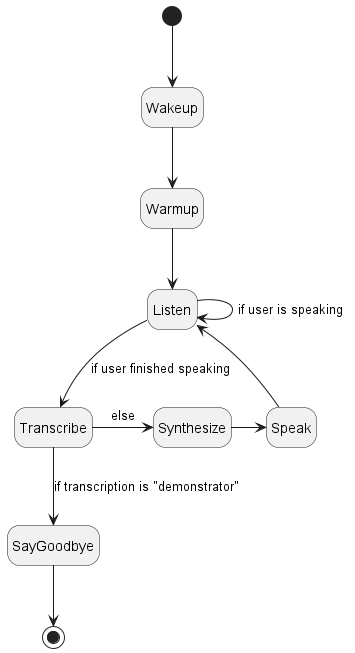
\includegraphics[width=0.5\textwidth]{../diagrams/state_app.png}
    \caption{State machine for a Demonstrator standalone app.}
    \label{fig:state_app}
\end{figure}
\newpage
\begin{figure}[h]
    \centering
    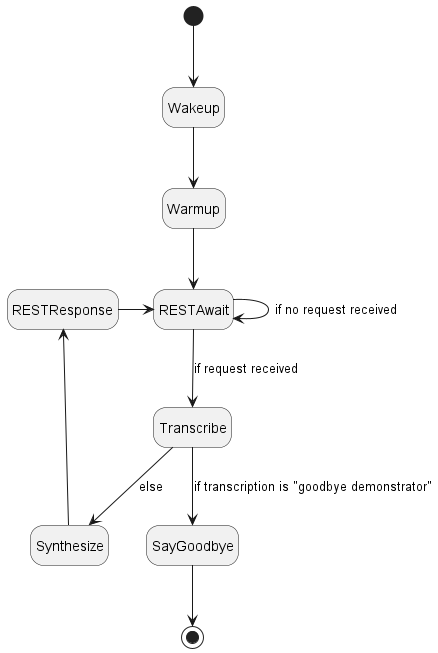
\includegraphics[width=0.6\textwidth]{../diagrams/state_server.png}
    \caption{State machine for a Demonstrator server.}
    \label{fig:state_server}
\end{figure}
\begin{figure}[h]
    \centering
    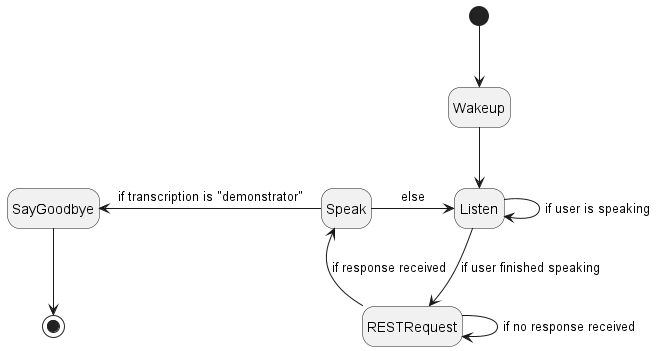
\includegraphics[width=0.9\textwidth]{../diagrams/state_client.png}
    \caption{State machine for a Demonstrator client.}
    \label{fig:state_client}
\end{figure}

\section{Files in Root}
This section describes the files that exist at the project root.

\subsection{\texttt{.env}}
The \texttt{.env} file in the root of the repository contains information about what kind of Demonstrator instance should be run.
It must include at least the following two constants:
\begin{itemize}
    \item DEMONSTRATOR\_MODE: in ["client", "server", "app"]. Defines what kind of Demonstrator should be run on this machine (should this machine act as a Demonstrator client or server, or should it run as a standalone app?).
    \item DEMONSTRATOR\_PROFILE: should match the name of a profile configured in the \texttt{/configs/demonstrator\_configs.yaml} folder. "default" is the default profile and thus the default value to be used here.
\end{itemize}
This file is not tracked by Git, as its contents should be independent for every Demonstrator install (otherwise, for example, all installations would start to act as a server after pulling new code).

\subsection{\texttt{.gitignore}}
The \texttt{.gitignore} file contains a list of files and folders that should not be tracked by Git.
At the top, there are the files and folders that should not be tracked that relate to the contents of specifically the Demonstrator repository, such as not tracking audio files.
Afterwards, standard templates from gitignore.io are used to not track files and folders that one typically does not want to track, such as files generated by LaTeX when building a PDF and the folder containing the Python environment.

\subsection{\texttt{README.md}}
The README that shows up when viewing the repository on a Git platform, such as GitHub.
It currently contains a brief overview of what the Demonstrator is and does, how it works, and how it can be run.

\subsection{\texttt{requirements.txt}}
This file contains all the Python package requirements for running the Demonstrator as a client, server, and standalone app.
It installs the CUDA (GPU) versions of the PyTorch packages by default instead of the CPU versions and automatically skips packages that cannot be installed on a specific OS, such as the Piper TTS on Windows.
By running the command \texttt{pip install -r requirements.txt}, the installation of all dependencies can be done automatically.
If the Demonstrator software is changed or expanded to use new or different packages, that should be reflected in the requirements.txt by keeping it up-to-date.
